\documentclass[11pt,letterpaper]{article}
\usepackage[T1]{fontenc}
\usepackage[utf8]{inputenc}
\usepackage[spanish]{babel}
\usepackage{lmodern}
\usepackage[margin=2.6cm]{geometry}
\usepackage{amsmath,booktabs,graphicx,placeins}
\usepackage[hidelinks]{hyperref}

% Completar con los datos del registro oficial de servicio social.
\newcommand{\alumno}{Ulises Abdiel Cabello Cárdenas}
\newcommand{\carrera}{Matemáticas}
\newcommand{\programa}{.}
\newcommand{\claveprograma}{.}
\newcommand{\dependencia}{.}
\newcommand{\responsable}{.}
\newcommand{\periodo}{.}
\newcommand{\horas}{.}

\begin{document}

\begin{titlepage}
\centering
{\Large\bfseries Universidad Nacional Autónoma de México\par}
\vspace{0.35cm}
{\large Facultad de Ciencias\par}
\vfill
{\LARGE\bfseries Informe final de servicio social\par}
\vspace{0.6cm}
{\Large Pronóstico de generación eléctrica horaria mediante modelos de regresión lineal\par}
\vfill
\begin{tabular}{@{}lp{0.59\textwidth}@{}}
\textbf{Prestador} & \alumno \\
\textbf{Licenciatura} & \carrera \\
\textbf{Programa} & \programa \\
\textbf{Clave} & \claveprograma \\
\textbf{Dependencia receptora} & \dependencia \\
\textbf{Responsable} & \responsable \\
\textbf{Periodo} & \periodo \\
\textbf{Horas acreditadas} & \horas \\
\end{tabular}
\vfill
Ciudad de México
\end{titlepage}

\section*{Informe final de actividades}
% hacerlo en primera persona colocar la imagen del mapa de la republica, se incluyo el preprocesamiento ... mas visualizaciones mejor.
\section{Introducción}

Durante mi servicio social preparé una serie horaria de generación eléctrica del área de Baja California (BCA) y comparé cuatro modelos de regresión para pronosticar la generación de la siguiente hora. Trabajé con los registros del Centro Nacional de Control de Energía (CENACE) utilizados en el proyecto de tesis.

Mi objetivo fue construir una comparación reproducible entre mínimos cuadrados ordinarios (OLS), Ridge, Lasso y Elastic Net. Utilicé OLS como referencia y examiné cómo cambió el error al incorporar regularización en ajustes con muchos rezagos y pocos ejemplos.

\section{Descripción de las actividades desarrolladas}

\subsection{Primera etapa: revisión y preparación de los datos}

En \texttt{datos.csv} identifiqué la marca temporal, el área y la generación eléctrica en MWh. Seleccioné el área BCA y los registros de 2022. Ordené los registros por fecha y conservé los primeros 6\,001, correspondientes al 70\,\% inicial de la serie. Dentro de ese subconjunto evalué los modelos mediante ventanas móviles.

Comprobé que cada ejemplo reuniera 24 observaciones previas y un valor objetivo separados por intervalos de una hora. Descarté las ventanas que atravesaban discontinuidades. Usé la fecha para ordenar los registros y verificar esa continuidad. Como entradas del comparador utilicé los 24 rezagos de generación y como respuesta tomé el valor observado en la hora siguiente.

\subsection{Segunda etapa: implementación de los modelos básicos}

En la comparación común, para pronosticar la generación $y_t$ se usaron los 24 valores observados de $y_{t-24}$ a $y_{t-1}$. Cada regresión estimó un intercepto $\beta_0$ y un coeficiente $\beta_j$ por rezago. Si $z_{t,j}$ es el rezago $j$ estandarizado con el promedio y la desviación del conjunto de entrenamiento de ese ajuste, el pronóstico toma la forma
\[
  \widehat y_t = \beta_0 + \sum_{j=1}^{24}\beta_j z_{t,j}.
\]
El intercepto recoge el nivel de la serie que estima el modelo cuando los rezagos estandarizados valen cero. Las penalizaciones se aplican a los coeficientes de los rezagos.

\paragraph{Mínimos cuadrados ordinarios (OLS).}
El ajuste minimiza $\sum_i (y_i-\widehat y_i)^2$ sobre los ejemplos de entrenamiento. Los errores grandes influyen más en la estimación por el uso del cuadrado. Cuando los rezagos contienen información muy parecida y hay pocos ejemplos, cambios pequeños en la ventana pueden producir coeficientes muy distintos. En este estudio, OLS sirve como referencia para medir el efecto de regularizar.

\paragraph{Ridge.}
Agrega una penalización proporcional a $\sum_j\beta_j^2$. Al penalizar con mayor intensidad los coeficientes de magnitud alta, permite repartir el peso entre rezagos relacionados y reduce la sensibilidad del ajuste. Para la prueba común se usó $\alpha=1.0$.

\paragraph{Lasso.}
Emplea una penalización proporcional a $\sum_j |\beta_j|$. El ajuste puede llevar algunos coeficientes exactamente a cero y dejar solo parte de los rezagos en la ecuación de pronóstico. Si varios rezagos son similares, la selección puede cambiar de una ventana a otra. En la prueba común se utilizó $\alpha=0.1$.

\paragraph{Elastic Net.}
Combina las penalizaciones absoluta y cuadrática. La primera permite excluir algunos rezagos y la segunda modera el peso de los que permanecen, incluso cuando varios están correlacionados. La comparación usó $\alpha=0.1$ y una proporción de $0.5$ para el componente $L_1$ bajo la parametrización del estimador.

Las implementaciones individuales del directorio \texttt{root} también se revisaron como parte del servicio social. Sus entradas, tamaños de ventana y parámetros se describen junto con las gráficas de la sección~\ref{sec:graficas-individuales}.


\subsection{Tercera etapa: evaluación y documentación}

En cada origen ajusté los cuatro modelos con los 24 ejemplos válidos más recientes disponibles en ese momento. Estimé los parámetros de estandarización con las entradas de entrenamiento de cada ajuste y mantuve los pronósticos en la escala original, en MWh.

Evalué los últimos 168 orígenes elegibles y obtuve, en cada uno, un pronóstico a una hora por modelo. Calculé las métricas sobre esas observaciones y tracé las series observadas y pronosticadas para examinar los errores.

\section{Resultados obtenidos}

\subsection{Componentes desarrollados}

Preparé la serie y construí ejemplos con rezagos horarios. Después comparé las cuatro regresiones con las mismas entradas, datos de entrenamiento y horas de evaluación. Finalmente reuní las métricas y las trayectorias observadas y pronosticadas. Los scripts y la documentación técnica están en el repositorio de tesis.\footnote{\href{https://github.com/UlisesACC/Tesis_unam}{Repositorio de la tesis en GitHub}.}

\subsection{Comparación de los pronósticos}

Usé el MAE para resumir el error absoluto promedio y el RMSE para dar más peso a los errores grandes. Ambas métricas se expresan en MWh. Con el coeficiente $R^2$ comparé la suma de errores cuadrados con la que obtendría si usara la media de las observaciones evaluadas como predicción constante.

\begin{table}[htbp]
\centering
\caption{Desempeño en 168 predicciones de generación eléctrica a una hora.}
\begin{tabular}{lrrr}
\toprule
Modelo & MAE (MWh) & RMSE (MWh) & $R^2$ \\
\midrule
OLS & 198.8016 & 285.1903 & -0.1096 \\
Ridge & 93.0581 & 118.6614 & 0.8079 \\
Lasso & 163.3162 & 226.1509 & 0.3023 \\
Elastic Net & \textbf{91.1626} & \textbf{116.3124} & \textbf{0.8154} \\
\bottomrule
\end{tabular}
\end{table}

Con Elastic Net obtuve los menores valores de MAE y RMSE. Con Ridge obtuve valores cercanos y observé que el MAE bajó de 198.80 MWh con OLS a 93.06 MWh. Con Lasso también registré errores menores que con OLS, aunque mayores que con Ridge y Elastic Net. El $R^2$ negativo de OLS indica que su error cuadrático superó al de la referencia constante en los orígenes que evalué.

\subsection{Comparación gráfica de la generación observada y pronosticada}

En la figura~\ref{fig:comparacion-modelos-lineales} reuní la generación observada y los pronósticos a una hora de los cuatro modelos. Mostré un acercamiento de aproximadamente el 12 al 15 de agosto de 2022 para revisar cómo respondió cada método a los cambios de generación en las mismas horas. Para las métricas de la tabla utilicé los 168 orígenes evaluados.

\begin{figure}[!htbp]
\centering
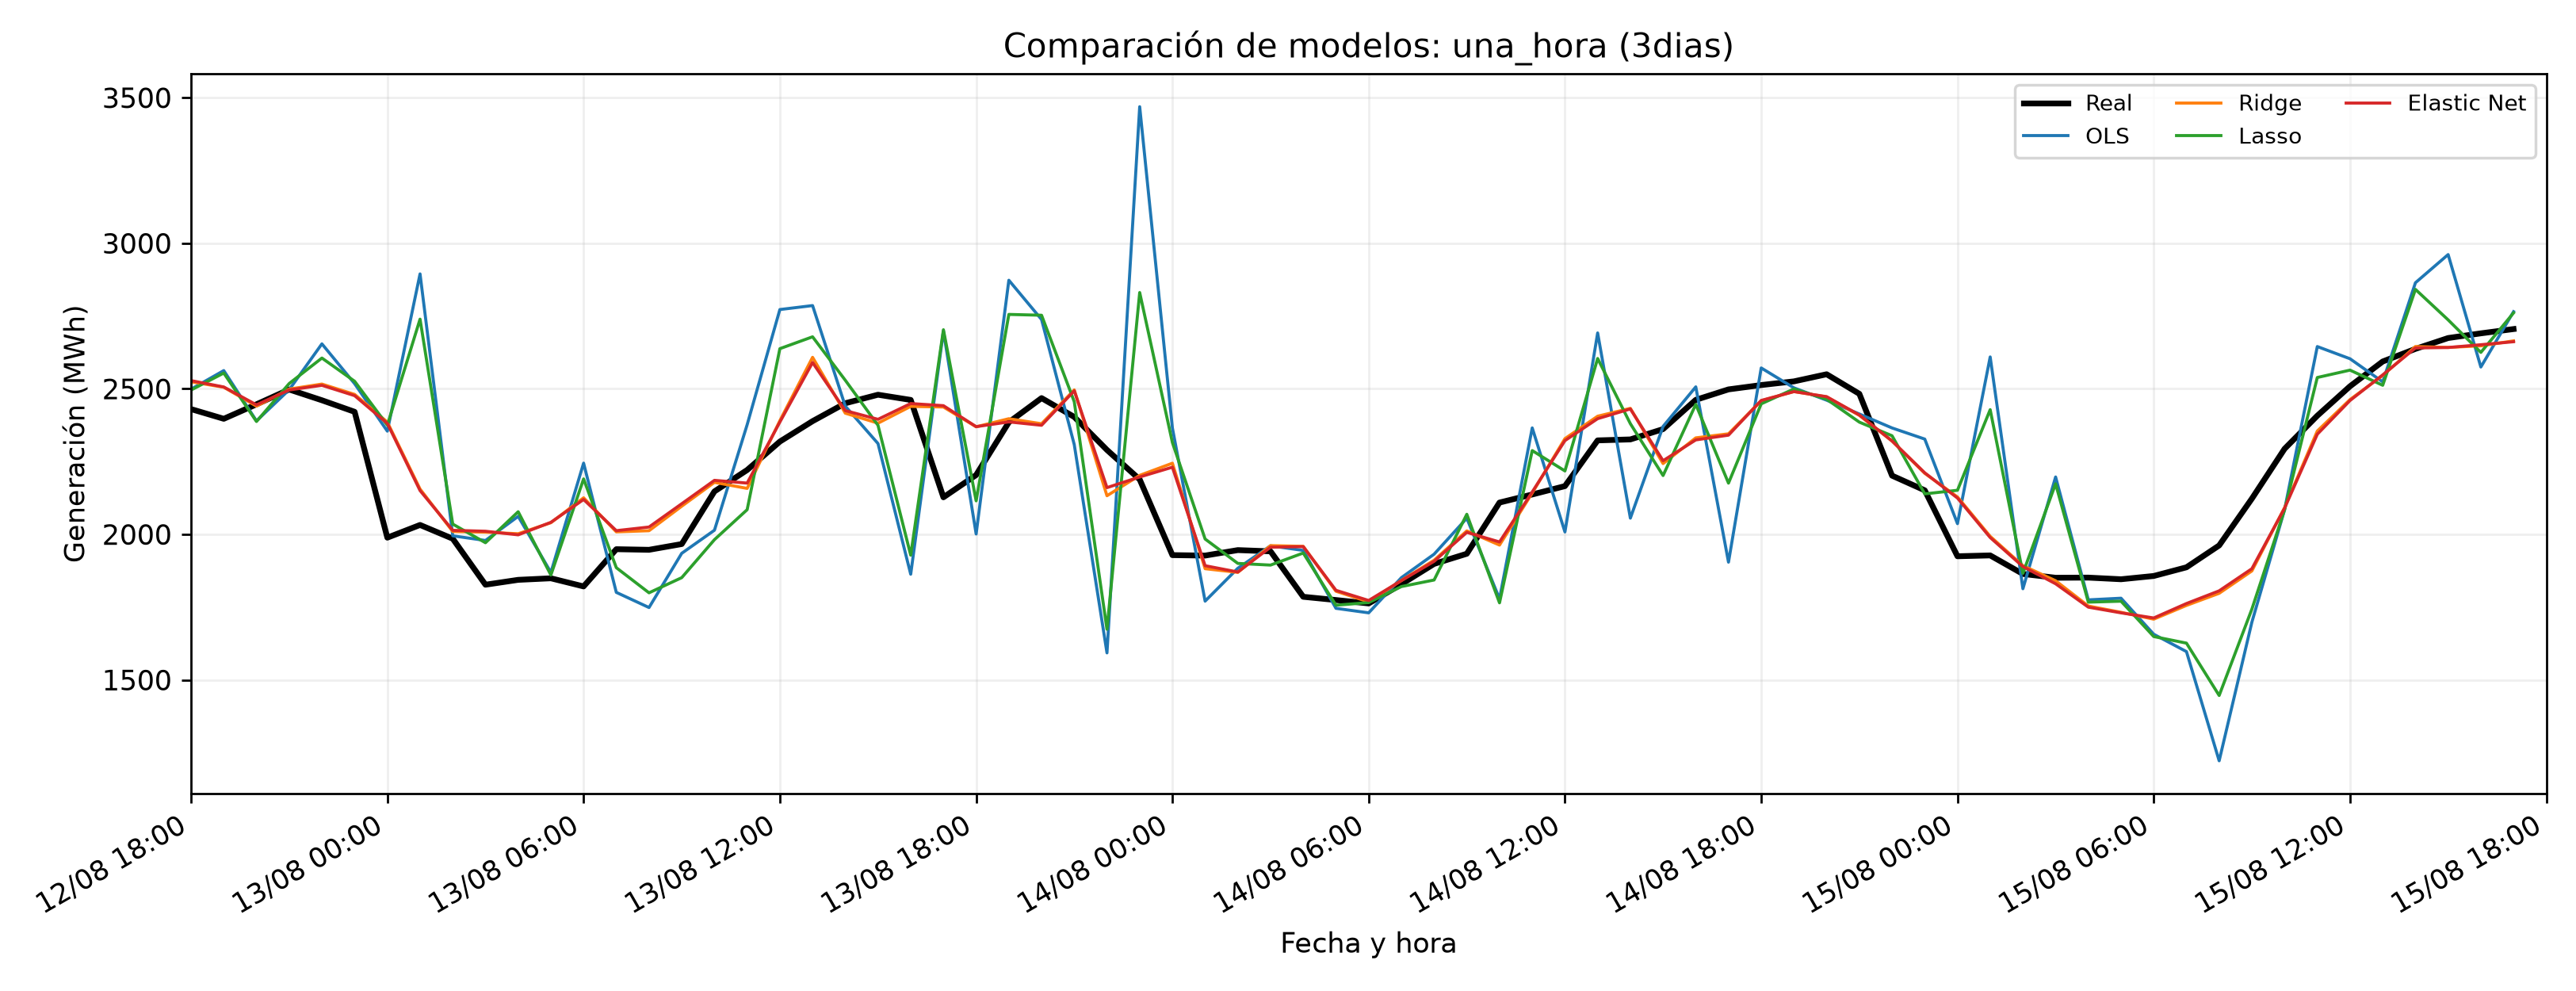
\includegraphics[width=\linewidth]{figuras/comparacion_una_hora_3dias.png}
\caption{Generación eléctrica observada y pronosticada por los cuatro modelos lineales en Baja California. Fuente: experimento de pronóstico a una hora del repositorio de tesis.}
\label{fig:comparacion-modelos-lineales}
\end{figure}

\FloatBarrier

\subsection{Gráficas de las implementaciones individuales}
\label{sec:graficas-individuales}

Las figuras de esta subsección se tomaron del directorio \texttt{codigos de docker/root} del repositorio de tesis. Muestran corridas individuales. La tabla de 168 pronósticos corresponde a la comparación común con 24 rezagos y 24 ejemplos de entrenamiento por ajuste. Las figuras individuales documentan la evolución de los métodos con sus propias configuraciones.

\paragraph{OLS con 24 rezagos.}
El script \texttt{OLS.py} filtra BCA durante 2022, conserva el primer 70\,\% de los registros ordenados y construye ejemplos con 24 rezagos consecutivos. Ajusta OLS con las 24 filas de entrenamiento anteriores a cada objetivo y estandariza las entradas en cada ajuste. La figura~\ref{fig:root-ols} amplía los primeros tres días desde el primer pronóstico válido. Las marcas de fecha y hora permiten ubicar cambios puntuales. La distancia vertical entre los puntos de la misma hora es el error absoluto en MWh. El 3 de enero, cerca del mediodía, el pronóstico baja hasta aproximadamente 400 MWh mientras la generación observada se mantiene por encima de 1\,300 MWh. El mismo día aparecen sobreestimaciones cercanas a 1\,900 MWh en la curva pronosticada. Este acercamiento permite ver errores de ambos signos dentro de una misma jornada.

\begin{figure}[!htbp]
\centering
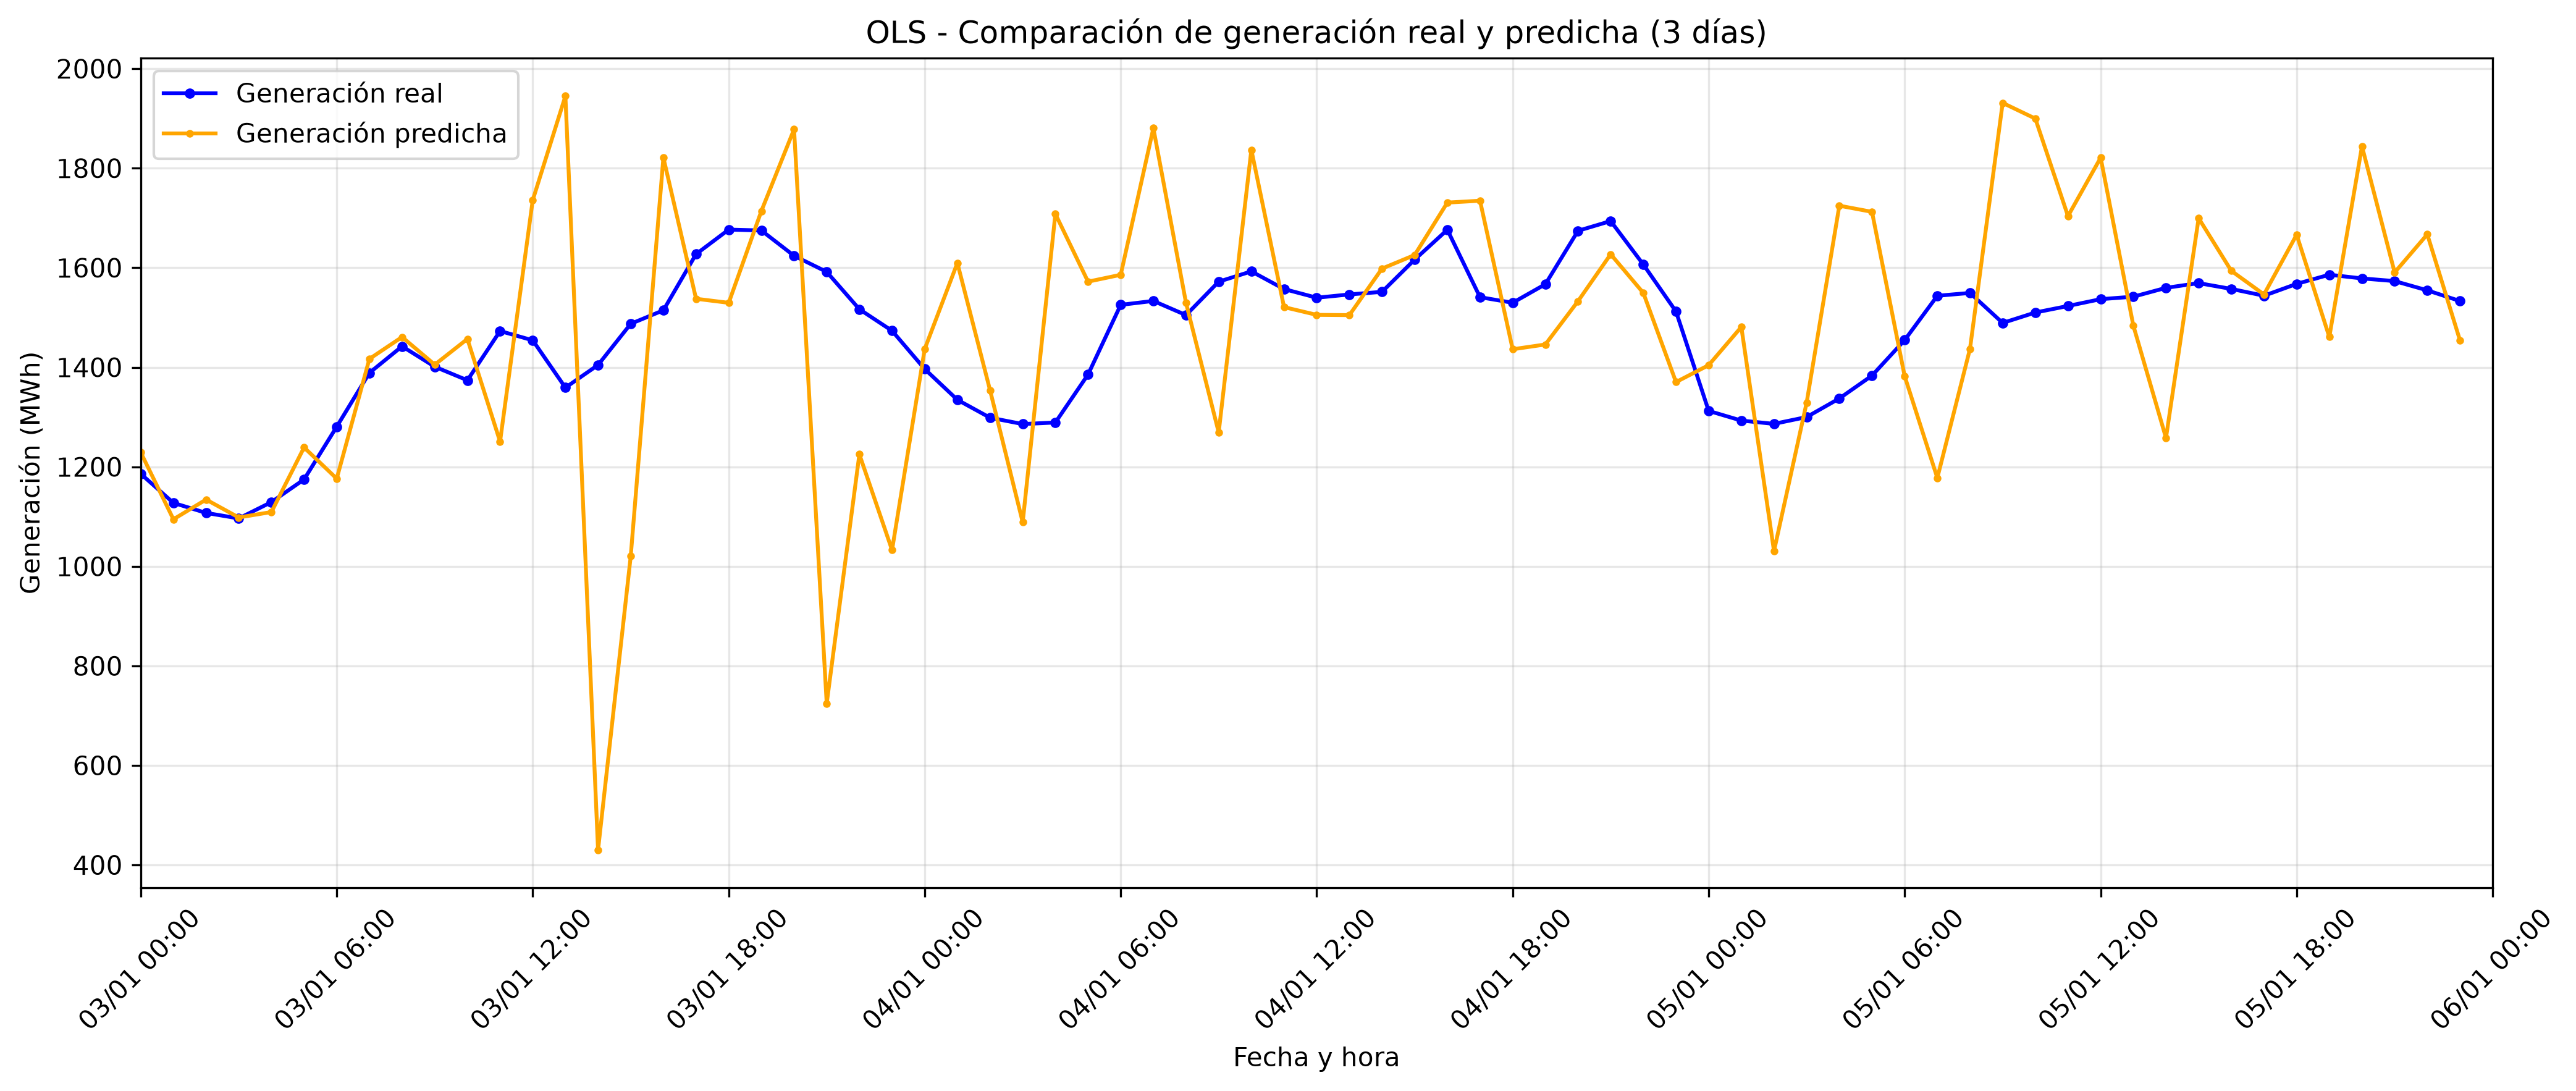
\includegraphics[width=\linewidth]{figuras/prediccion_vs_real_ols_3dias.png}
\caption{OLS. Generación observada y pronosticada durante los primeros tres días desde el inicio de la evaluación individual. Fuente: salida de \texttt{OLS.py}.}
\label{fig:root-ols}
\end{figure}
\FloatBarrier

\paragraph{Ridge, Lasso y Elastic Net con un rezago y calendario.}
Las tres implementaciones usan la generación del registro anterior y cinco variables de calendario\,: hora del día, día del año, año, mes y día de la semana. Cada ventana de 13 filas usa las primeras 12 para ajustar y la última para pronosticar. La selección de $\alpha$ se realiza por validación cruzada de tres particiones dentro de cada ventana con candidatos $0.001$, $0.01$, $0.1$, $1$ y $10$. Elastic Net también considera proporciones $L_1$ de $0.1$, $0.5$ y $0.9$. El eje horizontal de estas figuras enumera las predicciones sucesivas y el eje vertical indica la generación en MWh. El rezago corresponde a la fila previa de la serie filtrada. Si hay huecos en los registros, el avance de un índice puede abarcar más de una hora.

\paragraph{Ridge.}
En la figura~\ref{fig:root-ridge} se puede seguir si la predicción conserva el nivel general de generación y cuánto se aparta en picos y valles. La regularización cuadrática reduce la magnitud de los coeficientes, de modo que el efecto estimado de la fila previa y el calendario se mantiene moderado. Alrededor del índice 4\,000 se aprecia el paso a un nivel de generación más alto. La densidad de las curvas en ese tramo facilita ver el cambio de nivel, pero dificulta distinguir el error de cada observación.

\begin{figure}[!htbp]
\centering
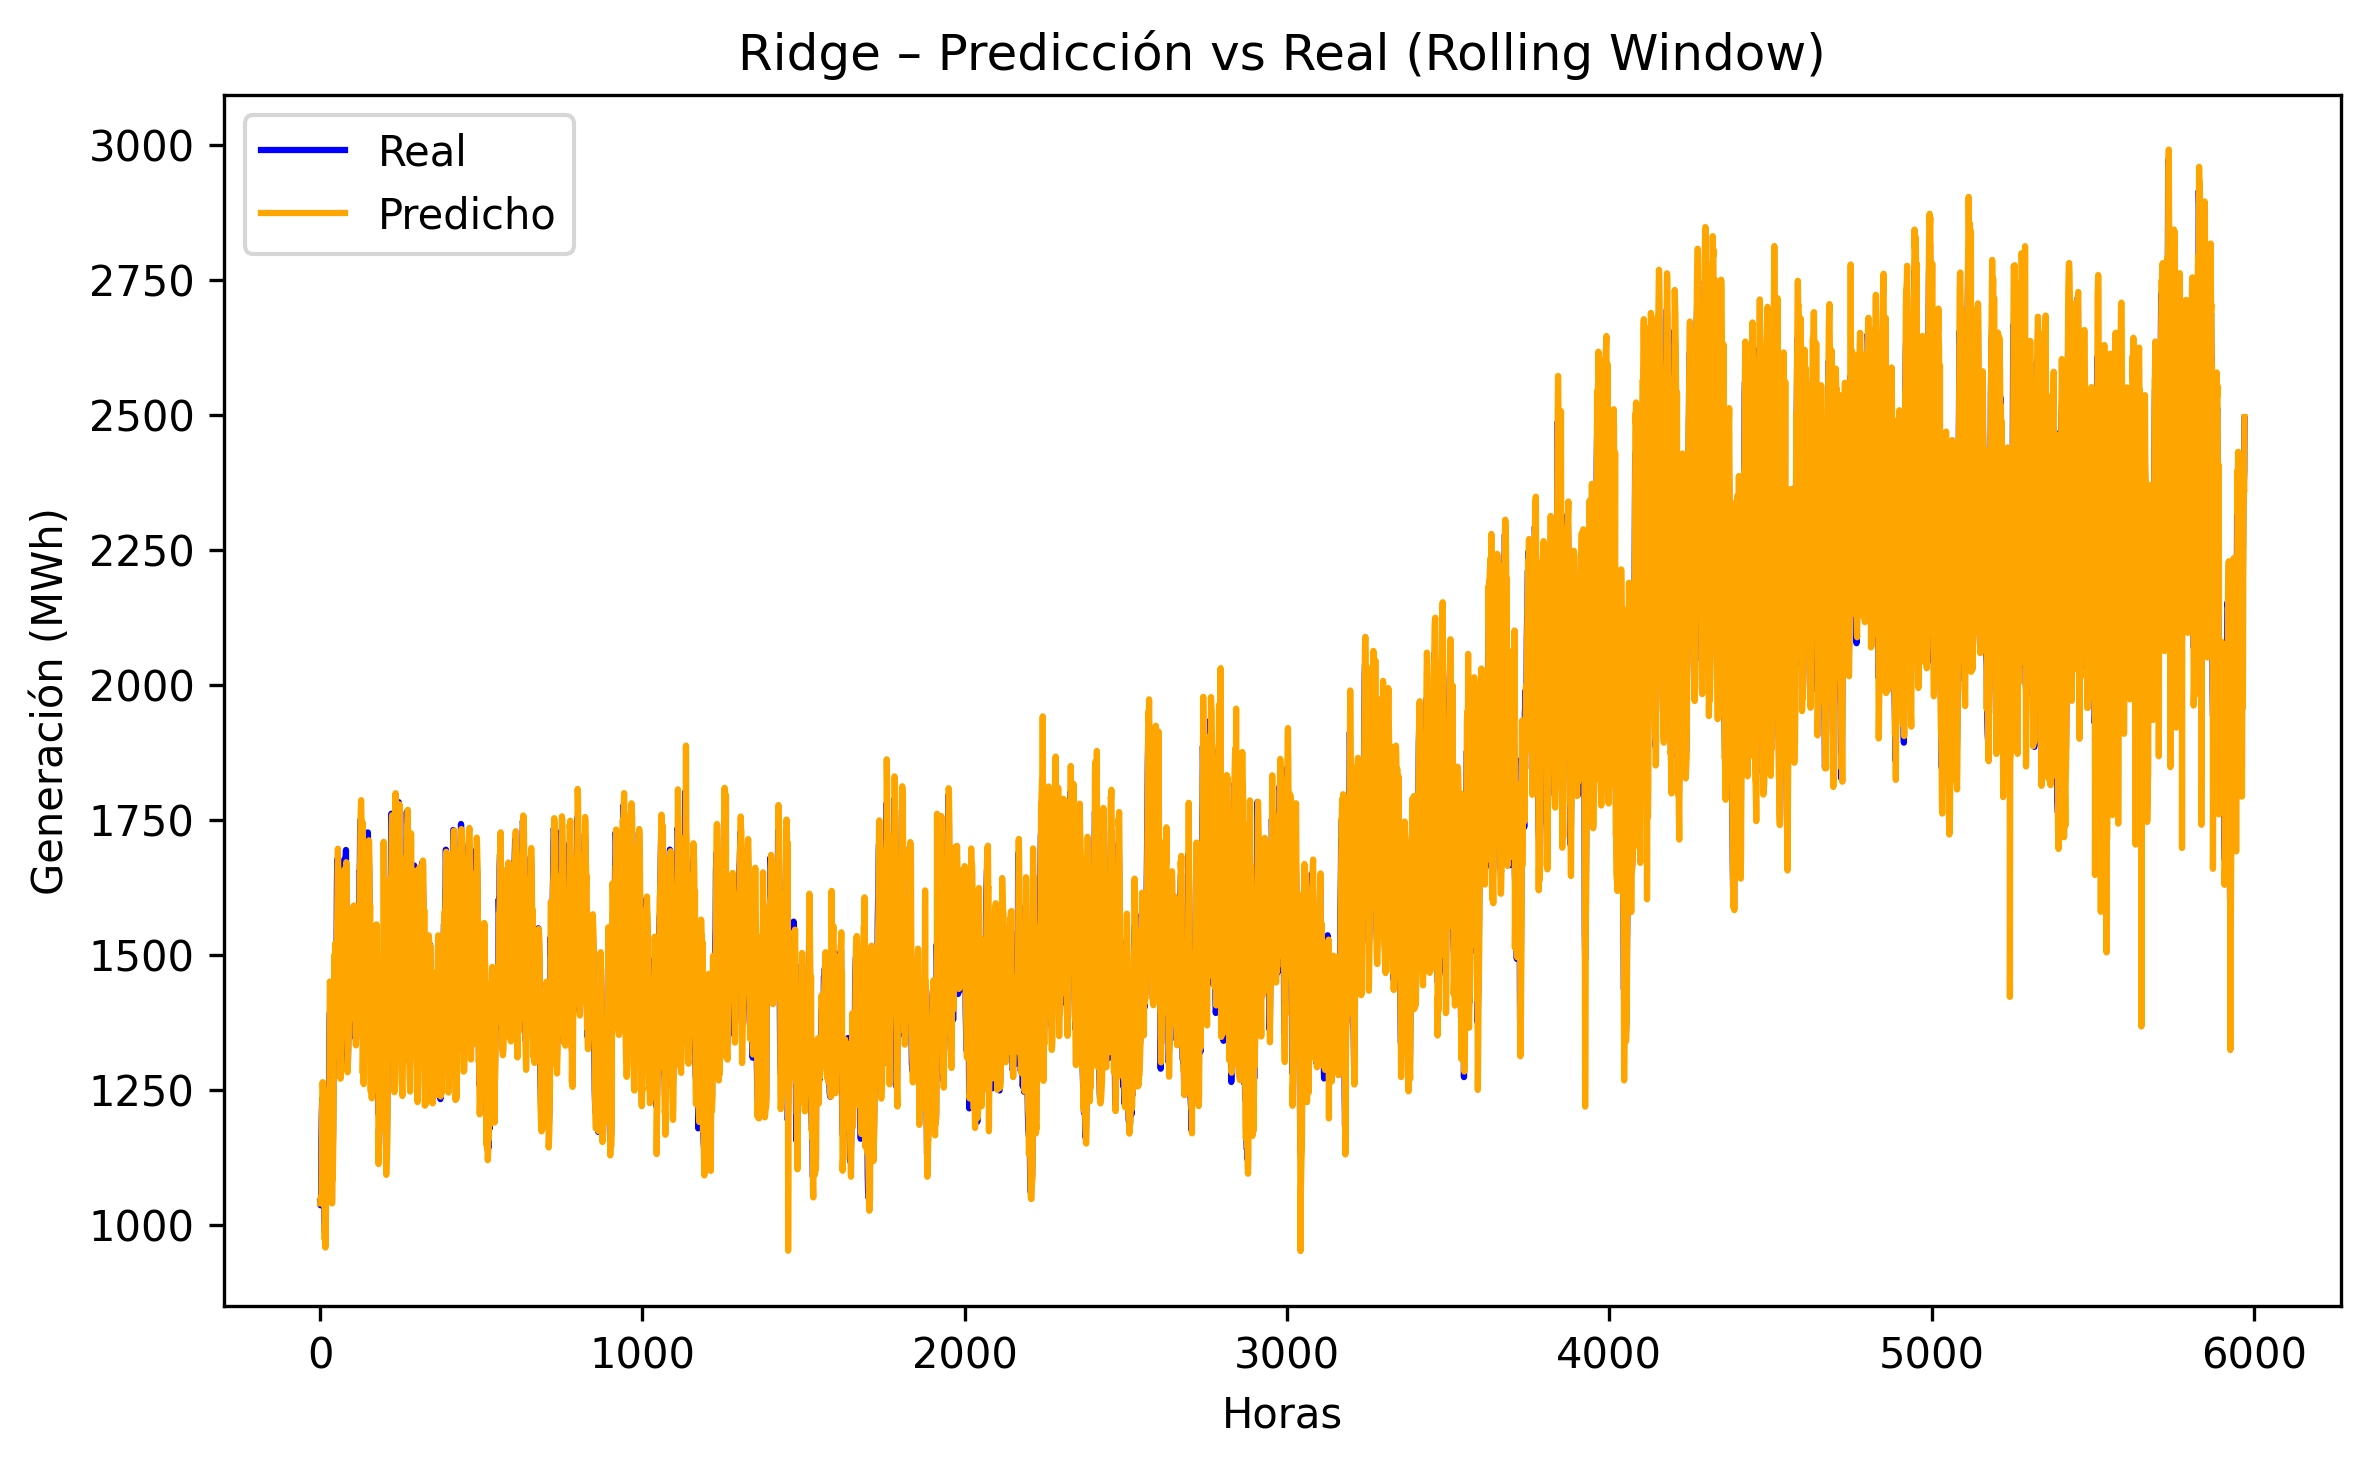
\includegraphics[width=0.88\linewidth]{figuras/prediccion_vs_real_ridge.png}
\caption{Ridge. Generación observada y pronosticada con un rezago y variables de calendario. Fuente: salida de \texttt{ridge.py}.}
\label{fig:root-ridge}
\end{figure}
\FloatBarrier

\paragraph{Lasso.}
La figura~\ref{fig:root-lasso} permite revisar si, después de la penalización absoluta, las predicciones acompañan los ascensos y descensos de la serie. A partir de aproximadamente 4\,000 predicciones, el rango de generación es más amplio y algunos máximos se acercan a 3\,000 MWh. Un acercamiento local facilitaría distinguir qué picos se sobreestiman y cuáles se subestiman. La figura presenta los pronósticos por ventana. Para identificar qué variables tuvieron coeficiente cero haría falta revisar los coeficientes de cada ajuste.

\begin{figure}[!htbp]
\centering
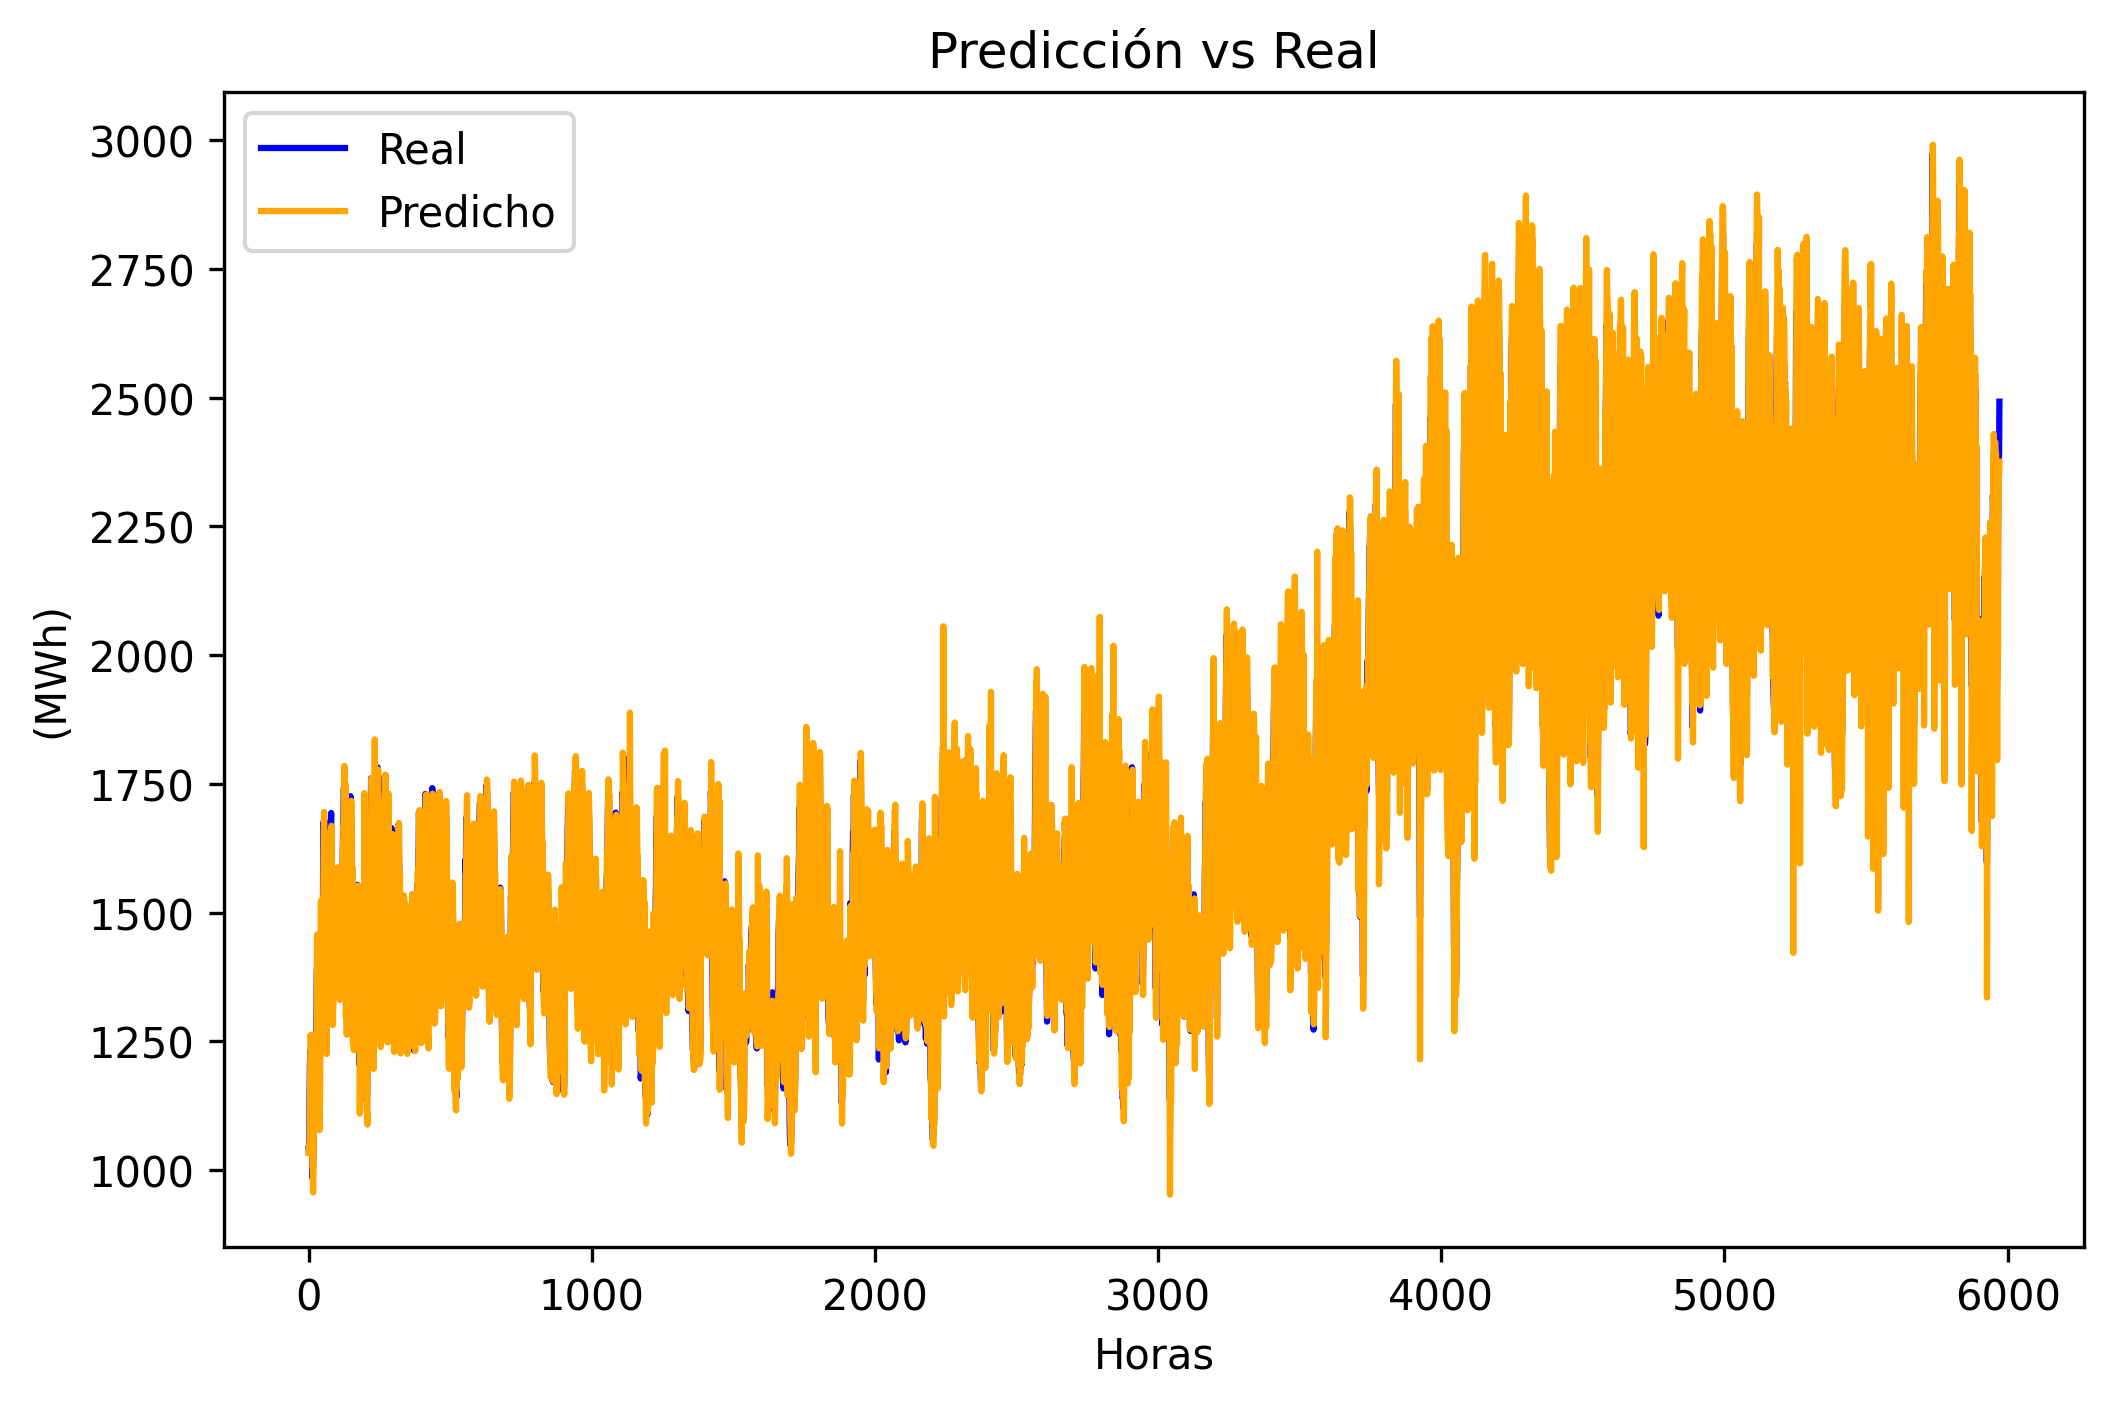
\includegraphics[width=0.88\linewidth]{figuras/prediccion_vs_real_lasso.png}
\caption{Lasso. Generación observada y pronosticada con selección de la penalización en cada ventana. Fuente: salida de \texttt{lasso.py}.}
\label{fig:root-lasso}
\end{figure}
\FloatBarrier

\paragraph{Elastic Net.}
En la figura~\ref{fig:root-elasticnet}, la cercanía entre curvas permite revisar el seguimiento de la generación a lo largo de las ventanas. En la primera parte del gráfico predominan valores entre 1\,000 y 2\,000 MWh. En el tramo final aparecen picos próximos a 3\,000 MWh. La trayectoria pronosticada acompaña ese aumento general del nivel, y la superposición a esta escala dificulta juzgar los errores puntuales. Como cada ajuste selecciona tanto la intensidad total de la penalización como la proporción absoluta, ese equilibrio puede variar durante la evaluación.

\begin{figure}[!htbp]
\centering
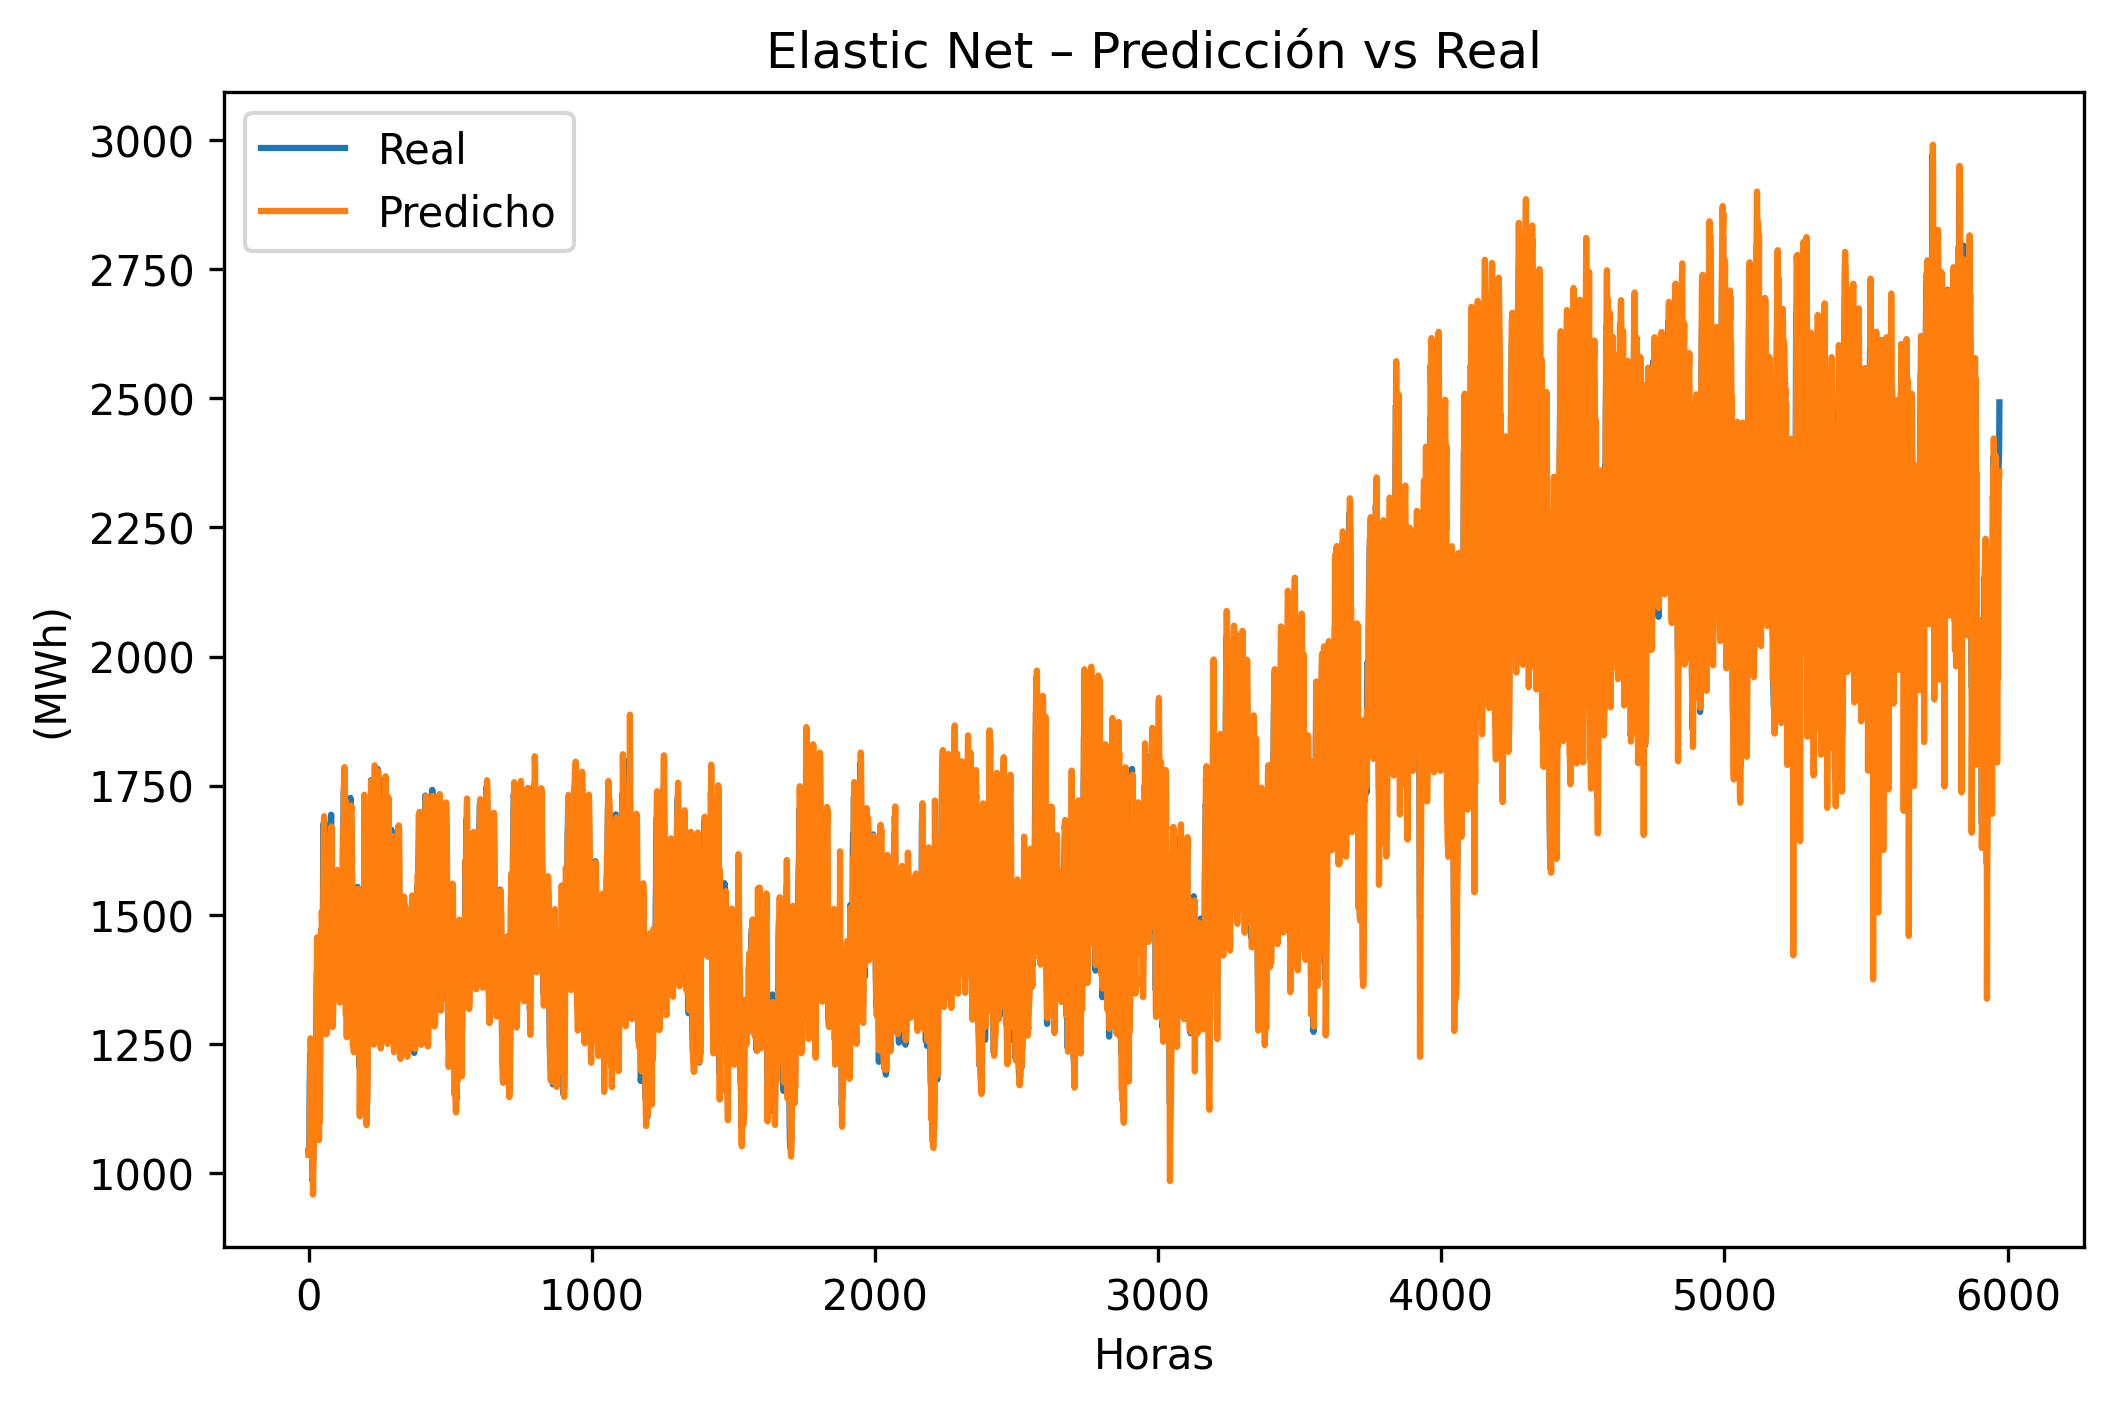
\includegraphics[width=0.88\linewidth]{figuras/prediccion_vs_real_elasticnet.png}
\caption{Elastic Net. Generación observada y pronosticada con penalización mixta ajustada en cada ventana. Fuente: salida de \texttt{Elastic Net.py}.}
\label{fig:root-elasticnet}
\end{figure}
\FloatBarrier


\section{Conclusiones}

Durante el servicio social apliqué métodos de regresión a una serie eléctrica real y evalué su desempeño bajo condiciones comparables. Al verificar la continuidad horaria me aseguré de que los rezagos representaran horas consecutivas. Con la ventana móvil ajusté cada pronóstico usando la información disponible en su origen.

En el escenario de Baja California de 2022 obtuve los menores errores con Ridge y Elastic Net. Observé este resultado con 24 rezagos, 24 ejemplos por ajuste y un horizonte de una hora. Mi conclusión se limita al periodo y a los orígenes que evalué.

\end{document}
